\section{Implementierung}

\subsection{GUI Komponenten}

Da die Hauptaufgabe dieser Projektarbeit darin bestand, die benötigten GUI Komponenten zu entwickeln und in richtiger Weise zusammenzusetzen, wird darauf im Folgenden detailliert eingegangen.

\subsubsection{ShortcutField}

Ein \emph{ShortcutField} ist -- wie in Abschnitt \ref{ui} bereits erwähnt -- für die Anzeige und Bearbeitung von Tastaturkürzeln zuständig. Sofern noch kein Shortcut eingegeben wurde, zeigt es zudem eine Aufforderung zum Eingeben eines Shortcuts in Form eines Texts an (\glqq enter shortcut...\grqq). Um diesen Anforderungen gerecht zu werden, setzt sie sich aus drei bereits bestehenden Komponenten zusammen: Für das Löschen des gesamten Shortcuts dient ein \emph{CrossButton} (umkreistes Kreuz), für die Anzeige und Bearbeitung des Shortcuts kommt die \emph{ShortcutView}-Komponente zum Einsatz und die Textaufforderung wird durch ein \emph{JLabel} realisiert.

\begin{figure}[H]
	\centering
	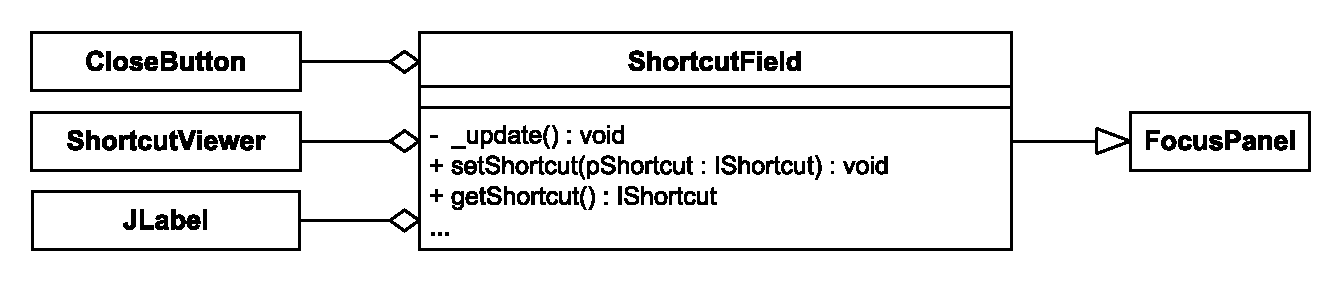
\includegraphics[width=0.8\linewidth]{../graphic/diagrams/CD_ShortcutField/ShortcutField}
	\caption{ShortcutField}
	\label{fig:shortcutfield}
\end{figure}

Die eigentliche Funktionalität wird durch die verwendeten Komponenten bereitgestellt. Das \emph{ShortcutField} kümmert sich selber lediglich um die Anzeige der jeweils richtigen Komponente (\emph{JLabel} oder \emph{ShortcutView}), sowie um das Horchen auf Tastatureingaben mittels eines \emph{KeyListeners}. Die private Methode \emph{\_update()} ist für das Ein- und Ausblenden der jeweiligen Komponente zuständig (siehe \autoref{fig:ShortcutField-update}). Sie wird initial und bei jeder Änderung des Shortcuts aufgerufen.

\vspace{20px}

\begin{wrapfigure}[11]{l}[0cm]{0.50\textwidth}
    \centering
	\vspace{-5px}
	\begin{spacing}{0.75}
		\begin{javacode}[firstnumber=205]
private void _update()
{
  boolean empty = getShortcut() == null;
	
  viewerContainer.setVisible(!empty);
  textContainer.setVisible(empty);
  
  crossButton.setVisible(isEditable());
  crossButton.setEnabled(!empty);
}		\end{javacode}
	\end{spacing}
	\caption{Ein- und Ausblenden der Komponenten}
	\label{fig:ShortcutField-update}
\end{wrapfigure}

Zunächst wird überprüft, ob das \emph{ShortcutField} leer ist (kein Shortcut gesetzt). Das Ergebnis dieser Überprüfung wird in der lokalen Variable \emph{empty} gespeichert. Anschließend werden die Sichtbarkeiten der Komponenten aktualisiert, wobei der \emph{ShortcutViewer} nur bei gesetztem und die Textaufforderung nur bei nicht gesetztem Tastenkürzel angezeigt wird. Der \emph{CrossButton} wird im Editiermodus immer angezeigt aber nur aktiviert, sobald ein Shortcut eingegeben wird.

\newpage

\subsubsection{Check-Button}

\vspace{-3px}

Um die Grundfunktionalität des im Abschnitt \ref{ui} erwähnten Check-Buttons zu definieren, wurde zunächst das Interface \emph{ICheckComponent} erstellt. Indessen wird festgelegt, dass ein Check-Button einen Checked-Zustand besitzt, welcher angibt, ob innerhalb der Komponente ein grüner Haken (\emph{true}) oder ein rotes Kreuz (\emph{false}) angezeigt werden soll (siehe \autoref{fig:cdcheckbutton}).

Die Klasse \emph{CheckToggleButton} implementiert das beschriebene Interface und erbt von der Swing Klasse \emph{JToggleButton}. Sie kümmert sich um das Einfügen und Aktualisieren des richtigen Symbols. Innerhalb von \emph{setChecked(...)} wird die private Methode \emph{\_updateIcon()} aufgerufen, welche ihrerseits das jeweilige Symbol über das gesetzte Icon zeichnet (siehe Anhang \ref{CheckToggleButton}). Insgesamt stellt ein \emph{CheckToggleButton} eine vollwertige CheckComponent dar, welche direkt verwendet werden könnte.

\begin{figure}[H]
	\centering
	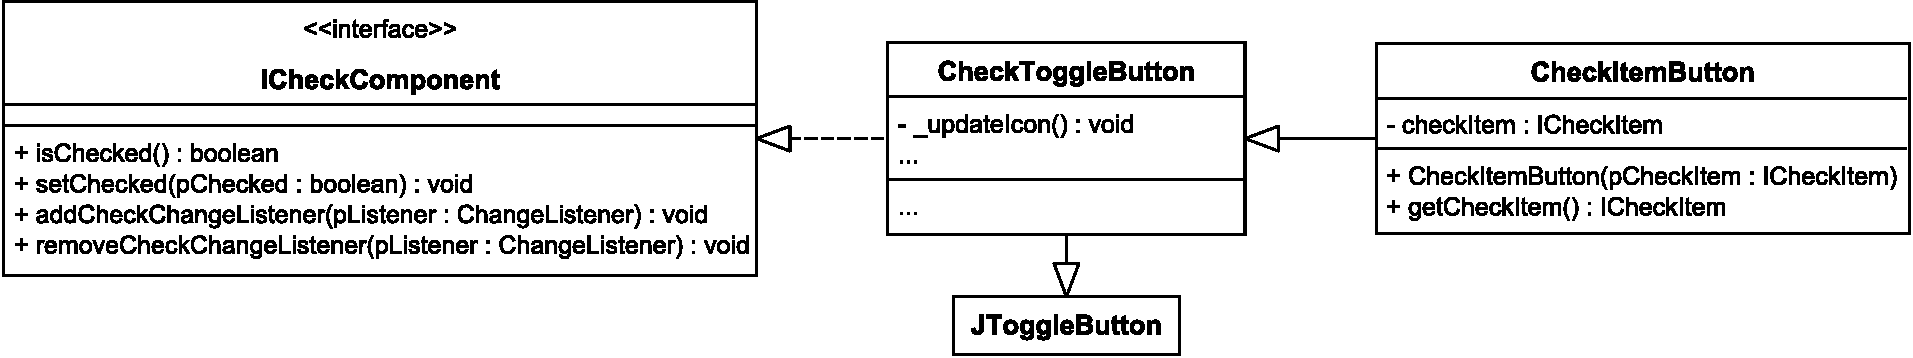
\includegraphics[width=1\linewidth]{../graphic/diagrams/CD_CheckButton/CD_CheckButton}
	\caption{CheckItemButton}
	\label{fig:cdcheckbutton}
\end{figure}

\vspace{-9px}

Um die Benutzung von \emph{CheckToggleButtons} innerhalb des Shortcut Editors bzw. im Zusammenhang mit \emph{ICheckItems} einfacher zu gestalten, wurde die Klasse \emph{CheckItemButton} eingeführt. Diese erweitert \emph{CheckToggleButton} und kann über den Konstruktor ein \emph{ICheckItem} aufnehmen. Wie im Anhang \ref{CheckItemButton} ersichtlich, werden innerhalb dieses Konstruktors alle Eigenschaften entsprechend dem \emph{ICheckItem} gesetzt (z. B. Checked-Zustand oder Icon).

\vspace{-9px}

\subsubsection{CheckItemContainer}

\vspace{-3px}

\begin{wrapfigure}[15]{r}[0cm]{165px}
	\vspace{-12px}
	\centering
	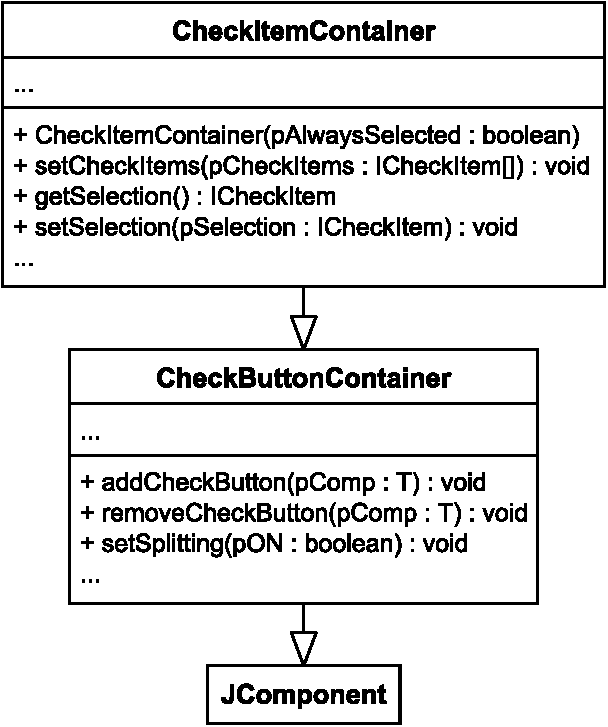
\includegraphics[width=.95\linewidth]{../graphic/diagrams/CD_CheckItemContainer/CD_CheckItemContainer}
	\caption{CheckItemContainer}
	\label{fig:cdcheckitemcontainer}
\end{wrapfigure}

Der Designentwurf lässt erkennen, dass die Check-Buttons einer bestimmten Positionierung bzw. Sortierung unterliegen: Auf der linken Seite befinden sich alle unchecked und auf der rechten Seite alle checked Buttons. Zudem wird bei den Check-Buttons zur Auswahl des Browsers ein Abstand zwischen den beiden Buttongruppen eingefügt. 

Um diese Positionierung zu realisieren, wurde der \emph{CheckItemContainer} erstellt. Dieser stellt eine \emph{JComponent} dar, welcher mittels eines \emph{BoxLayouts} seine CheckButtons horizontal nebeneinander ausrichtet. Um den zuvor erwähnten Abstand ein- und auszuschalten, existiert die Methode \emph{setSplitting(...)}, welche einen \emph{boolean} erwartet. Ändert sich der Checked-Zustand eines CheckButtons, so kümmert sich der Container auch um die richtige Umsortierung.

Um wiederum die Nutzung innerhalb des Shortcut Editors zu erleichtern, existiert der \emph{CheckItemContainer}. Diesem kann man \emph{CheckItems} setzten (\emph{setCheckItems(...)}), wonach dieser intern die benötigten Check-Buttons erzeugt und sich selbst hinzufügt oder Unnötige wieder entfernt (siehe Anhang \ref{CheckItemContainer}). Zudem kann über die Methode \emph{getSelection()} der aktuell selektierte Check-Button ausgelesen werden.

\subsubsection{CheckItemAccordion}

\vspace{-8px}

Die Accordion-Komponente ist in der Lage, einen konkreten Pfad des Datenmodells für Browsertestergebnisse mit allen verfügbaren Details darzustellen (siehe \autoref{fig:uxDesigns}).
Jede Sektion des Accordions visualisiert genau ein CheckItem. Sofern Untersektionen vorhanden sind, wird zusätzlich ein CheckItemContainer angezeigt. Dieser dient zur Navigation durch das Datenmodell, wobei immer genau das CheckItem dargestellt wird, welches in der vorherigen Sektion ausgewählt ist.

\begin{wrapfigure}[10]{l}[0cm]{230px}
	\vspace{-12px}
	\centering
	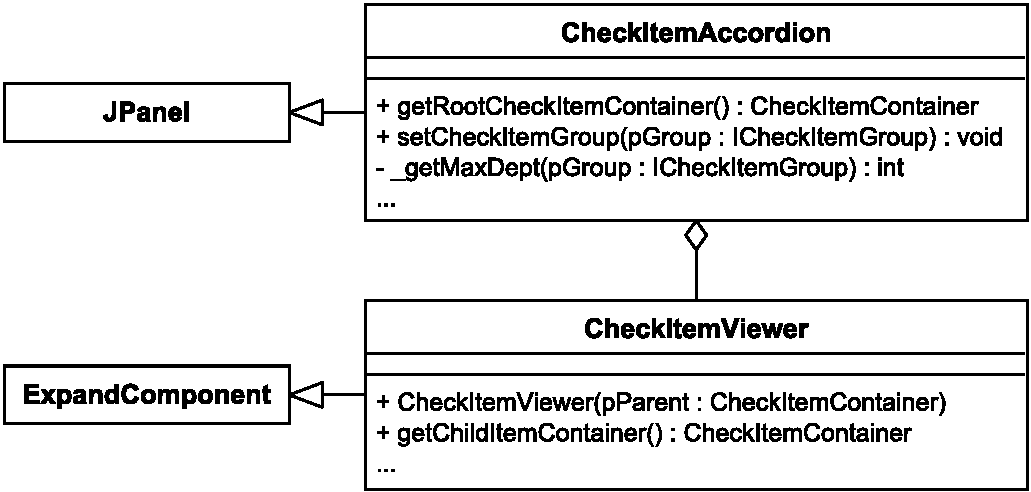
\includegraphics[width=0.95\linewidth]{../graphic/diagrams/CD_CheckItemAccordion/CheckItemAccordion}
	\caption{CheckItemAccordion}
	\label{fig:checkitemaccordion}
\end{wrapfigure}


Das \emph{CheckItemAccordion} erbt von der Swing Klasse \emph{JPanel} (siehe \autoref{fig:checkitemaccordion}) und verwendet zur vertikalen Positionierung der einzelnen Sektionen das \emph{BoxLayout}. Im Konstruktor wird der oberste \emph{CheckItemContainer} erzeugt, welcher zur Auswahl des Browsers dient und sich nicht innerhalb des Accordions befindet (siehe \autoref{fig:uxDesigns}). Um auf diesen außerhalb zugreifen zu können, dient die Methode \emph{getRootCheckItemContainer()}.

Eine Sektion wird durch die Klasse \emph{CheckItemViewer} repräsentiert (siehe \autoref{fig:checkitemaccordion}). Diese Komponente besitzt die Fähigkeit, alle Details eines CheckItems in tabellarischer Form darzustellen. Sie erbt von \emph{ExpandComponent}, wodurch die Funktion des Ein- und Ausklappens und die Anzeige einer Header-Leiste ermöglicht wird. Damit das selektierte \emph{CheckItem} des vorherigen \emph{CheckItemViewers} angezeigt und auf Selektionsänderungen reagiert werden kann, wird im Konstruktor der vorherige \emph{CheckItemContainer} übergeben. Diesem wird ein Listener hinzugefügt, welcher auf Änderungen der Selektion horcht und so die Aktualisierung des Viewers ermöglicht.

\begin{wrapfigure}[16]{r}[0px]{322px}
    \centering
	\vspace{-5px}
	\begin{spacing}{0.75}
		\begin{javacode}[firstnumber=62]
public void setCheckItemGroup(ICheckItemGroup pRootGroup)
{
  if(!Objects.equals(pRootGroup, rootGroup))
  {
    rootGroup = pRootGroup;
    
    rootCheckItemContainer.setCheckItems(pRootGroup.getItems());
    
    int dept = _getMaxDept(pRootGroup);
    CheckItemContainer children = rootCheckItemContainer;
    
    removeAll();
    for (int i = 0; i < dept; i++)
    {
      CheckItemViewer viewer = new CheckItemViewer(children);
      children = viewer.getChildItemContainer();
      add(viewer);
    }
  }
}\end{javacode}
	\end{spacing}
	\caption{Setzten der CheckItemGroup im CheckItemAccordion}
	\label{fig:CheckItemAccordion-setCheckItemGroup}
\end{wrapfigure}

In \autoref{fig:CheckItemAccordion-setCheckItemGroup} ist der Sourcecode der Methode \emph{setCheckItemGroup(...)} abgebildet. In dieser wird anhand der übergebenen \emph{ICheckItemGroup} das Accordion aufgebaut. Zu Beginn wird überprüft, ob es sich bei der übergebenen Gruppe um die bereits gesetzte handelt. Ist dies der Fall, so wird die Methode ohne Änderungen verlassen. Andernfalls werden dem RootCheckItemContainer die CheckItems der RootGruppe (Browser Check-Items) gesetzt. Anschließend wird über die Methode \emph{\_getMaxDept(...)} die maximale Tiefe der Baumstruktur von \emph{pRootGroup} ermittelt. Dieses Ergebnis dient als Grundlage für die Anzahl von Sektionen, die eingefügt werden. Nach dem Löschen aller vorhandenen Komponenten wird in jedem Schleifendurchgang eine Sektion eingefügt. Dabei wird im Konstruktor des \emph{CheckItemViewers} immer der \emph{CheckItemContainer} der vorherigen Sektion oder am Anfang der \emph{rootCheckItemContainer} übergeben. Dadurch wird der richtige Zusammenhang zwischen den Sektionen hergestellt.

\subsubsection{BreadCrumb und TreeTable}

Die Komponenten BreadCrumb und TreeTable mussten im Zuge dieser Projektarbeit nicht neu entwickelt werden, da sie bereits zu einem früheren Zeitpunkt umgesetzt wurden. 

\begin{wrapfigure}[12]{l}[0cm]{230px}
	\vspace{-12px}
	\centering
	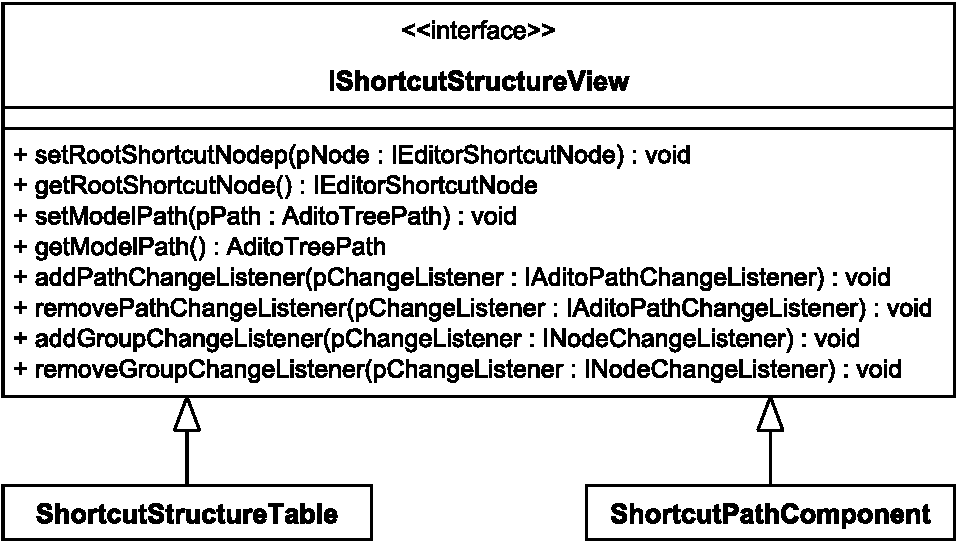
\includegraphics[width=1\linewidth]{../graphic/diagrams/CD_IShortcutStructureView/IShortcutStructureView}
	\caption{IShortcutStructureView}
	\label{fig:ishortcutstructureview}
\end{wrapfigure}

Um sie jedoch im Zusammenhang mit dem MVP-Architekturmuster verwenden zu können, mussten sie in eigene Klassen gekapselt werden, welche \emph{IShortcutStructureView} (siehe \autoref{fig:ishortcutstructureview}) implementieren. Dazu wurden die Klassen \emph{ShortcutPathComponent} (BreadCrumb) und \emph{ShortcutStructureTable} (TreeTable) erstellt (siehe Anhang \ref{ShortcutStructureTable} und \ref{ShortcutPathComponent}). Über die im Interface enthaltenen Methoden erhält die jeweilige Komponente ihre Informationen, welche zur Darstellung benötigt werden. Außerdem erhält sie die Möglichkeit, Wertänderungen über Listener zu kommunizieren. Wählt der Benutzer beispielsweise einen anderen Knoten in der BreadCrumb aus, so werden alle hinzugefügten \emph{PathChangeListener} informiert.


\subsubsection{ShortcutEditorUI}

Nach Implementierung der einzelnen Komponenten mussten diese zu einem gesamten User Interface zusammengesetzt werden. Hierzu wurde die Klasse \emph{ShortcutEditorUI} (siehe Anhang \ref{ShortcutEditorUI}) erstellt. Sie implementiert das Interface \emph{IShortcutEditorUI}, welches wiederum von \emph{IShortcutStructureView} erbt. Zudem erbt die UI von der Swing Klasse \emph{JPanel} (\autoref{fig:shortcuteditorui}).

\begin{figure}[H]
	\centering
	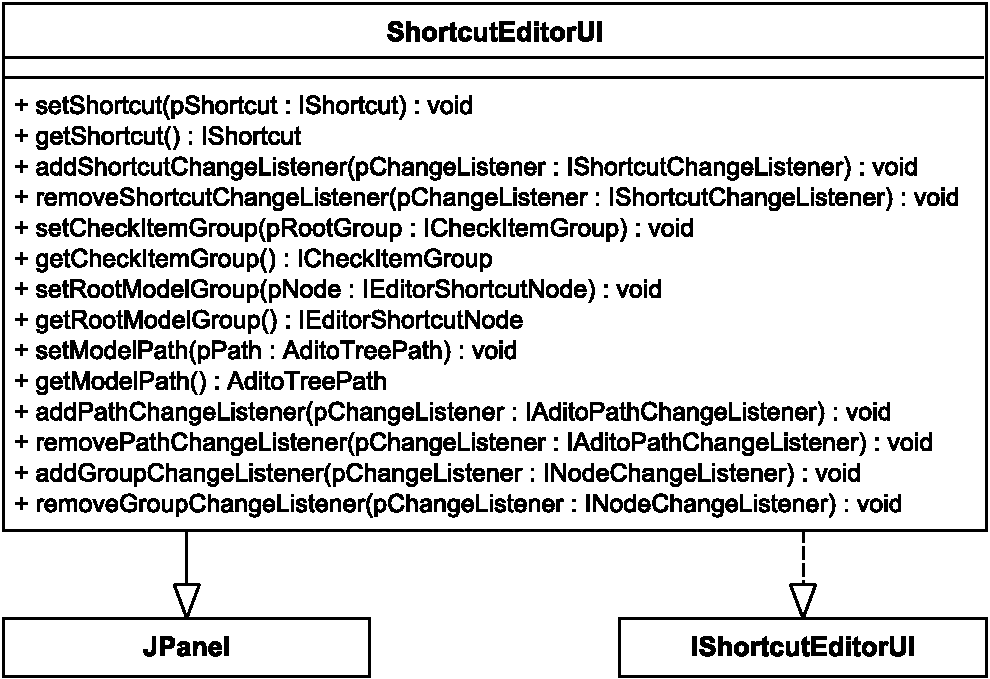
\includegraphics[width=1\linewidth]{../graphic/diagrams/CD_ShortcutEditorUI/ShortcutEditorUI}
	\caption{ShortcutEditorUI}
	\label{fig:shortcuteditorui}
\end{figure} 

\vspace{-12px}

Zur Anordnung der einzelnen Komponenten kommt das \emph{TableLayout} zum Einsatz. Im Konstruktor der Klasse werden die Spalten- und Zeilenausdehnungen des Layouts definiert und die Komponenten in die entsprechenden Zellen eingefügt. Außerdem werden das \emph{ShortcutStructureModel} und der \emph{ShortcutStructurePresenter} initialisiert. 

Da die Funktionalität in den für die UI verwendeten Komponenten enthalten ist, werden alle Getter- und Setter-Anfragen sowie die Listener direkt an das entsprechende Element (Komponente oder Model) weitergeleitet. In der \emph{setShortcut(...)} Methode der ShortcutEditorUI wird beispielsweise sofort die \emph{setShortcut(...)} Methode des ShortcutFields aufgerufen und so der zu setzende Shortcut direkt weitergegeben.

\newpage

\subsection{Presenter}

Folgend wird die Implementierung der im Abschnitt \ref{Architekturdesign} beschriebenen Presenter erläutert.

\subsubsection{ShortcutEditorPresenter}

\begin{wrapfigure}[11]{r}[0cm]{230px}
	\vspace{-12px}
	\centering
	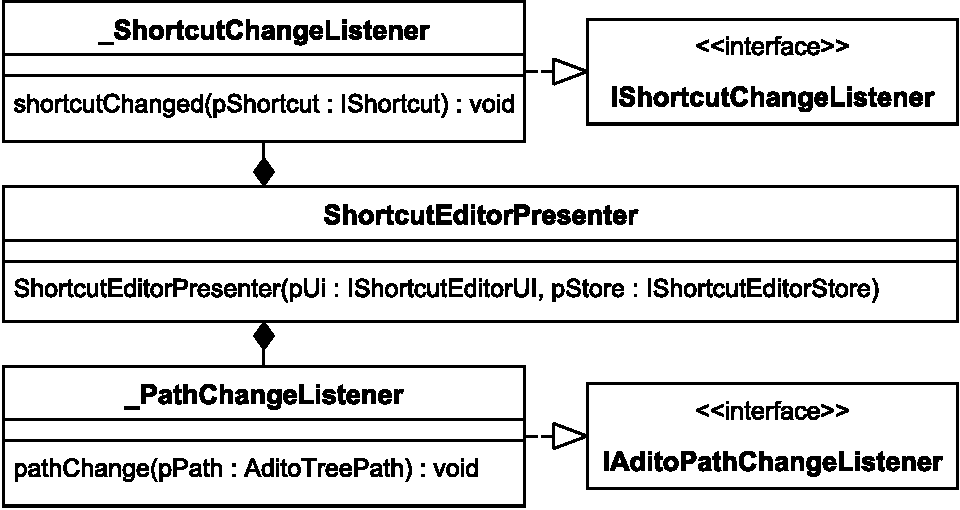
\includegraphics[width=230px]{../graphic/diagrams/CD_ShortcutEditorPresenter/ShortcutEditorPresenter}
	\caption{ShortcutEditorPresenter}
	\label{fig:shortcuteditorpresenter}
\end{wrapfigure}

Um die Daten der \emph{ShortcutEditorUI} mit den in Abschnitten \ref{DatenmodellFunc} und \ref{DatenmodellBrow} beschriebenen Datenmodellen abzugleichen, existiert gemäß des MVP-Architekturmusters der \emph{ShortcutEditorPresenter} (siehe Anhang \ref{ShortcutEditorPresenter}). Diesem wird über den Konstruktor sowohl der Datenstore als auch eine \emph{IShortcutEditorUI} übergeben. Anschließend werden die UI Listener hinzugefügt, welche auf Shortcut- und Pfadänderungen horchen.

Ändert der Benutzer über die UI den Shortcut, so wird dieser in das entsprechende Datenmodell übertragen. Wird durch den Benutzer der Pfad geändert, also eine andere Aktion selektiert, so lädt der Presenter das Datenmodell der neuen Aktion. Zukünftige Shortcutänderungen werden dann in dieses Datenmodell übertragen.

\subsubsection{ShortcutStructurePresenter}

Da bei den beiden Komponenten TreeTable und BreadCrumb dieselben Daten präsentiert werden, kommt zur Abgleichung ebenfalls das MVP-Architekturmuster zum Einsatz, wobei die beiden genannten Komponenten die Views darstellen. Der Presenter (siehe Anhang \ref{ShortcutStructurePresenter}) erhält über den Konstruktor ein \emph{ShortcutStructureModel} und eine beliebige Anzahl von \emph{IShortcutStructureViews}. 

In \autoref{fig:ishortcutstructureview} wird ersichtlich, dass eine View einen \emph{IEditorShortcutNode} und einen \emph{AditoTreePath} besitzt. Der \emph{IEditorShortcutNode} hält die in Abschnitt \ref{DatenmodellFunc} beschriebene Baumstruktur der Aktionen und der Pfad gibt an, welcher Knoten des Baums selektiert ist. Über Änderung dieser Attribute informieren Listener, welche der View über die entsprechenden Methoden hinzugefügt werden können (z. B. \emph{addPathChangeListener(...)}). Da das \emph{ShortcutStructureModel} die gleiche Funktionalität benötigt, wie die View, implementiert es auch das Interface \emph{IShortcutStructureView} (siehe Anhang \ref{ShortcutStructureModel}).

Im Konstruktor des \emph{ShortcutStructurePresenters} (siehe Anhang \ref{ShortcutStructurePresenter}) werden sowohl dem Model als auch den einzelnen Views Pfad- und Node-Listener hinzugefügt. Löst ein Listener des Models aus, so werden die Änderungen in alle Views übertragen. Löst ein Listener einer View aus, so werden die Änderungen in das Model übertragen. Da dadurch wiederum der Listener des Models anschlägt, werden auch die anderen Views aktualisiert. So wird gewährleistet, dass alle Views und das Model zu jedem Zeitpunkt die gleichen Informationen besitzen.

\begin{figure}[H]
	\centering
	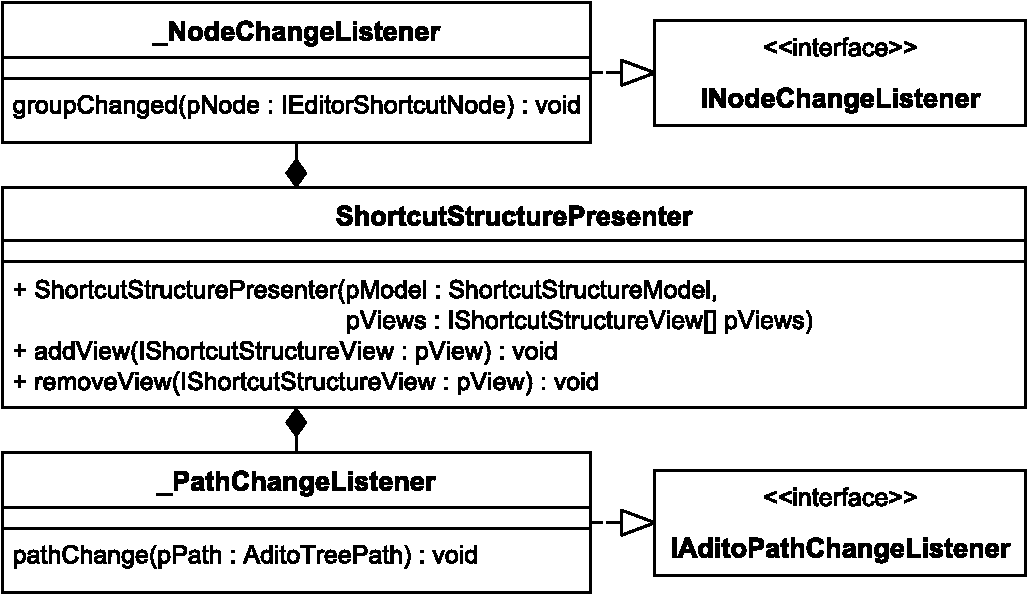
\includegraphics[width=0.6\linewidth]{../graphic/diagrams/CD_ShortcutStructurePresenter/ShortcutStructurePresenter}
	\caption{ShortcutStructurePresenter}
	\label{fig:shortcutstructurepresenter}
\end{figure}

\newpage